\begin{activity} \label{A:10.4.11} In what follows, we find the linearization of several different functions that are given in algebraic, tabular, or graphical form.
\ba

\item Find the linearization $L(x,y)$ for the function $g$ defined by 
$$
g(x,y) = \frac{x}{x^2+y^2}
$$
at the point $(1,2)$.  Then use the linearization to estimate the value of
 $g(0.8, 2.3)$.

\item Table \ref{T:10.4.wind.chill} provides a collection of
  values of the wind chill $w(v,T)$, in degrees Fahrenheit, as a
  function of  wind speed, in miles per hour, and temperature, also in degrees Fahrenheit.
 

\begin{table}[ht] 
  \begin{center}
    \begin{tabular}{|c||c|c|c|c|c|c|c|c|c|c|c|}
      \hline
      $v \backslash T$  
         &-30  &-25 &-20 &-15 &-10 &-5  &0   &5   &10  &15  &20  \\
      \hhline{|=|=|=|=|=|=|=|=|=|=|=|=|}
      5  &-46	&-40 &-34 &-28 &-22 &-16 &-11 &-5 &1 &7 &13  \\
      \hline
      10 &-53	&-47 &-41 &-35 &-28 &-22 &-16 &-10 &-4 &3 &9   \\
      \hline
      15 &-58	&-51 &-45 &-39 &-32 &-26 &-19 &-13 &-7 &0 &6  \\
      \hline
      20 &-61	&-55 &-48 &-42 &-35 &-29 &-22 &-15 &-9 &-2 &4  \\
      \hline
      25 &-64	&-58 &-51 &-44 &-37 &-31 &-24 &-17 &-11 &-4 &3 \\
      \hline
      30 &-67	&-60 &-53 &-46 &-39 &-33 &-26 &-19 &-12 &-5 &1 \\
      \hline
      35 &-69	&-62 &-55 &-48 &-41 &-34 &-27 &-21 &-14 &-7 &0 \\
      \hline
      40 &-71	&-64 &-57 &-50 &-43 &-36 &-29 &-22 &-15 &-8 &-1 \\
      \hline
    \end{tabular}
    \caption{Wind chill as a function of wind speed and temperature.}
    \label{T:10.4.wind.chill}
  \end{center}
\end{table}
%\begin{table}[ht]
%  \begin{center}
%    \begin{tabular}{|c||c|c|c|c|c|c|c|c|c|c|c|}
%      \hline
%      $v \backslash T$  
%         &-30  &-25 &-20 &-15 &-10 &-5  &0   &5   &10  &15  &20  \\
%      \hhline{|=|=|=|=|=|=|=|=|=|=|=|=|}
%      5  &-35  &-31 &-26 &-20 &-15 &-11 &-6  &1   &7   &12  &16  \\
%      \hline
%      10 &-58  &-52 &-45 &-38 &-31 &-27 &-22 &-15 &-9  &-2  &2   \\
%      \hline
%      15 &-70  &-65 &-60 &-51 &-45 &-40 &-33 &-25 &-18 &-11 &-6  \\
%      \hline
%      20 &-81  &-76 &-68 &-60 &-52 &-46 &-40 &-32 &-24 &-17 &-9  \\
%      \hline
%      25 &-89  &-83 &-75 &-67 &-58 &-52 &-45 &-37 &-29 &-22 &-15 \\
%      \hline
%      30 &-94  &-87 &-78 &-70 &-63 &-56 &-49 &-41 &-33 &-26 &-18 \\
%      \hline
%      35 &-98  &-90 &-83 &-72 &-67 &-60 &-52 &-43 &-35 &-27 &-20 \\
%      \hline
%      40 &-101 &-94 &-87 &-76 &-69 &-62 &-54 &-45 &-36 &-29 &-22 \\
%      \hline
%    \end{tabular}
%    \caption{Wind chill as a function of temperature and wind speed}
%    \label{T:10.2.wind.chill}
%  \end{center}
%\end{table}


Use the data to first estimate the appropriate partial derivatives, and then find the linearization $L(v,T)$ at the point $(25,-10)$.  Finally, use the linearization to estimate $w(25,-12)$, $w(23,-10)$, and $w(23,-12)$.

\item Figure \ref{F:10.4.activity.contour} gives a contour
  plot of a differentiable function $f$.  

  \begin{figure}[ht]
    \begin{center}
      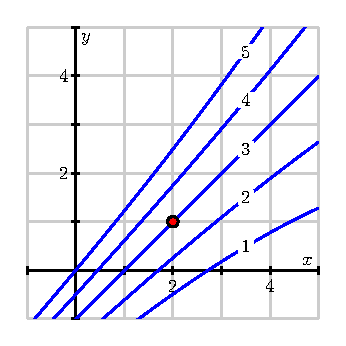
\includegraphics{figures/fig_10_3_activity_contour.eps}
    \end{center}
    \caption{A contour plot of $f(x,y)$.}
    \label{F:10.4.activity.contour}
  \end{figure}

  After estimating appropriate partial derivatives, determine the linearization $L(x,y)$ at the point $(2,1)$, and use it to
  estimate $f(2.2, 1)$, $f(2, 0.8)$, and $f(2.2, 0.8)$.



\ea

\end{activity}

\begin{activitySolution}
\ba
\item To find the linearization of $g$ we need the first order partials. Now
\begin{align*}
g_x(x,y) &= \frac{(x^2+y^2)-2x^2}{(x^2+y^2)^2} = \frac{y^2-x^2}{(x_2+y^2)^2} \\
g_y(x,y) &= \frac{-2xy}{(x^2+y^2)^2}.
\end{align*}
So the linearization of $g$ at the point (1,2) is
\[L(x,y) = g(1,2) +g_x(1,2)(x-1) + g_y(1,2)(y-2) = \frac{1}{5} + \frac{3}{25}(x-1) - \frac{4}{25}(y-2).\]
It follows that 
\[g(0.8,2.3) \approx L(0.8,2.3) = \frac{1}{5} - \frac{3}{25}(0.2) - \frac{4}{25}(0.3) = 0.128.\]
Since $g(0.8,2.3) \approx 0.135$, we have a fair approximation. This should be expected since the step sizes of 0.2 and 0.3 are not that small. 
\item We need $w_v(25,-10)$ and $w_T(25,-10)$ to find the linearization. Using the symmetric difference quotients gives us
\begin{align*}
w_v(25,-10) &\approx \frac{w(30,-10)-w(20,-10)}{10} = \frac{-39-(-35)}{10} = -0.4 \\
w_T(25,-10) &\approx \frac{w(25,-5)-w(25,-15)}{10} = \frac{-31-(-44)}{10} = 0.7.
\end{align*}  
So the linearization of $w$ at $(25, -10)$ is 
\[L(v,T) \approx -37 - 0.4(v-25) + 0.7(T+10).\]
Thus,
\begin{align*}
w(25,-12) &\approx L(25,-12) \approx -37 - 0.4(0) + 0.7(-2) = -38.4 \\
w(23, -10) &\approx L(23,-10) \approx -37 - 0.4(-2) + 0.7(0) = -36.2 \\
w(23, -12) &\approx L(23,-12) \approx -37 - 0.4(-2) + 0.7(-2) = -37.6.
\end{align*}

\item We need $f_x(2,1)$ and $f_y(2,1)$ to find the linearization. Using the symmetric difference quotients gives us
\begin{align*}
f_x(2,1) &\approx \frac{f(3,1)-f(1,1)}{2} \approx \frac{1.9-4.8)}{2} = -1.45 \\
f_y(2,1) &\approx \frac{f(2,2)-f(2,0)}{2} \approx \frac{4.3-1.8}{10} = 1.25.
\end{align*}  
So the linearization of $f$ at $(2, 1)$ is 
\[L(x,y) \approx 3 - 1.45(x-2) + 1.25(y-1).\]
Thus,
\begin{align*}
f(2.2,1) &\approx L(2.2,1) \approx 3 - 1.45(0.2) + 1.25(0) = 2.71 \\
f(2, 0.8) &\approx L(2, 0.8) \approx 3 - 1.45(0) + 1.25(-0.2) = 2.75 \\
f(-1.8, 2.1) &\approx L(2.2, 0.8) \approx 3 - 1.45(0.2) + 1.25(-0.2) = 2.46.
\end{align*}
The last two should be poor approximations since we are approximating quite far from the base point of $(2,1)$.
\ea
\end{activitySolution}

\aftera
